%TODO : REMOVE THIS
% --------------------------------------------------
\section{OBSOLETE, WRITE ONCE YOU'RE SURE. Area of residual distribution regions of interest}
% --------------------------------------------------
\label{appendix:systematics_bin_size}
% Edit count: 1

%TODO Include that x-track max uncertainty is 37 mm so that puts a minimum on the area bin width.
% DO I NEED TO EXPLAIN THIS IN MATH? I tried on June 3rd in my notes, it's complicated for such a simple thing.
% If this flies, you'll need to establish that reference frame == two fixed layers' frame as jargon in your thesis.
% Also need to establish x == perpendicular to wires; y == perpendicular to strips. ==> How do I do this consistently?
% May need to add 3100V reference if it's not already defined in your thesis.
% Define ROI as short form?
\textit{This is the reasoning as of 2021-08-10}.
Several factors went into choosing the area of the region of interest. First, the uncertainty in the cosmics tracks in the x-coordinates for the least geometrically favourable case was just under \SI{40}{\milli\meter}, so the width of the bin in x had to be larger. Also since the x-coordinate was discrete the number of entries in each bin was smoothed out by making the width in x larger than two wire groups, or \SI{72}{\milli\meter}. Second, the scale on which local offsets vary by more than \SI{50}{\micro\meter} is \SI{500}{\milli\meter}, assuming a large but possible rotation angle on a layer of \SI{1000}{\micro\radian}. Variations of \SI{50}{\micro\meter} were deemed significant since the desired position resolution of the quadruplet is \SI{100}{\micro\meter}. Therefore, the area had to be significantly lesser than \SI{500}{\milli\meter}. Third, the x-ray gun only covered an area of \SI{20}{\milli\meter} by \SI{20}{\milli\meter}, so ideally only cosmics tracks in that region would be included in the calculation of the mean. However, \SI{20}{\milli\meter} in $x$ was too small and the number of tracks is limited in small bins. Balancing these considerations, \SI{100}{\milli\meter} by \SI{100}{\milli\meter} bins were used. The variation in differences between cosmics residual means for these bins and \SI{40}{\milli\meter} by \SI{20}{\milli\meter} bins was insignificant thanks to the increased statistical uncertainty on the cosmics residual means for the smaller bins.

\textit{This section is outdated, and likely needs to be removed}

%TODO : How do I cite the distribution of rotations angles by Dylan?
The area of the region of interest in which to include tracks is primarily motivated by the misalignment model: the width of the region should be less than the scale on which the local offset is expected to change significantly. Changes in offset of order \SI{50}{\micro\meter}, the approximate position resolution of the sTGCs in the $\eta$-coordinate, are significant. In a misalignment model with an offset and rotation, only the rotation changes the local offset with respect to the x-coordinate \footnote{The effect of rotation can be modeled by assuming the recorded track position is related to the hit position by a passive rotation. The angle of rotation is the relative angle between the layer of interest and the nominal geometry. The local offset does change with respect to the track's y coordinate as well, but negligibly in the limit of small rotation angles.}.  The distribution of the as-built cathode board rotation angles shows that the RMS of the rotation angle is \SI{200}{\micro\radian} [https://indico.cern.ch/event/1035057/ PG. 18]; however, the distribution has a long tail so a typical rotation angle of \SI{1000}{\micro\radian} was used here. A rotation of \SI{1000}{\micro\radian} will cause a \SI{50}{\micro\meter} change in local offset over a change in x of \SI{50}{\centi\meter}. Therefore, the width of the region of interest should be less than \SI{500}{\milli\meter}.

Two other factors inform the width of the region. First, since the hits' x-coordinates are discrete the width in x must be larger than the pitch of the wire groups to ensure the bin will have a sufficient number of tracks fall in it. Second, more tracks will be included in a larger area so more statistics will be available for the residual distribution fit. For the bin widths wider than two wire groups, the statistics are sufficient. For each x-ray residual, the mean cosmics residual was calculated for a few different bin widths, and the difference in means plotted. Figure~\ref{fig:area_bin_size_mean_diff} shows an example for QL2.C.4. The width of the distribution is on the order of \SI{50}{\micro\meter}, showing that the calculation of the residual mean is relatively robust with respect to the area of the bin. However, \SI{50}{\micro\meter} is greater than the typical statistical uncertainty on the cosmic residual of means, which ranges from \SI{10}{\micro\meter} - \SI{40}{\micro\meter} depending on the tracking combination under study. Therefore, the cosmic residual means are assigned an uncertainty of \SI{50}{\micro\meter}.
%TODO : Verity that you actually apply the 50 um uncertainty.

%TODO : This figure should have the mean and rms on it.

\begin{figure}
    \centering
    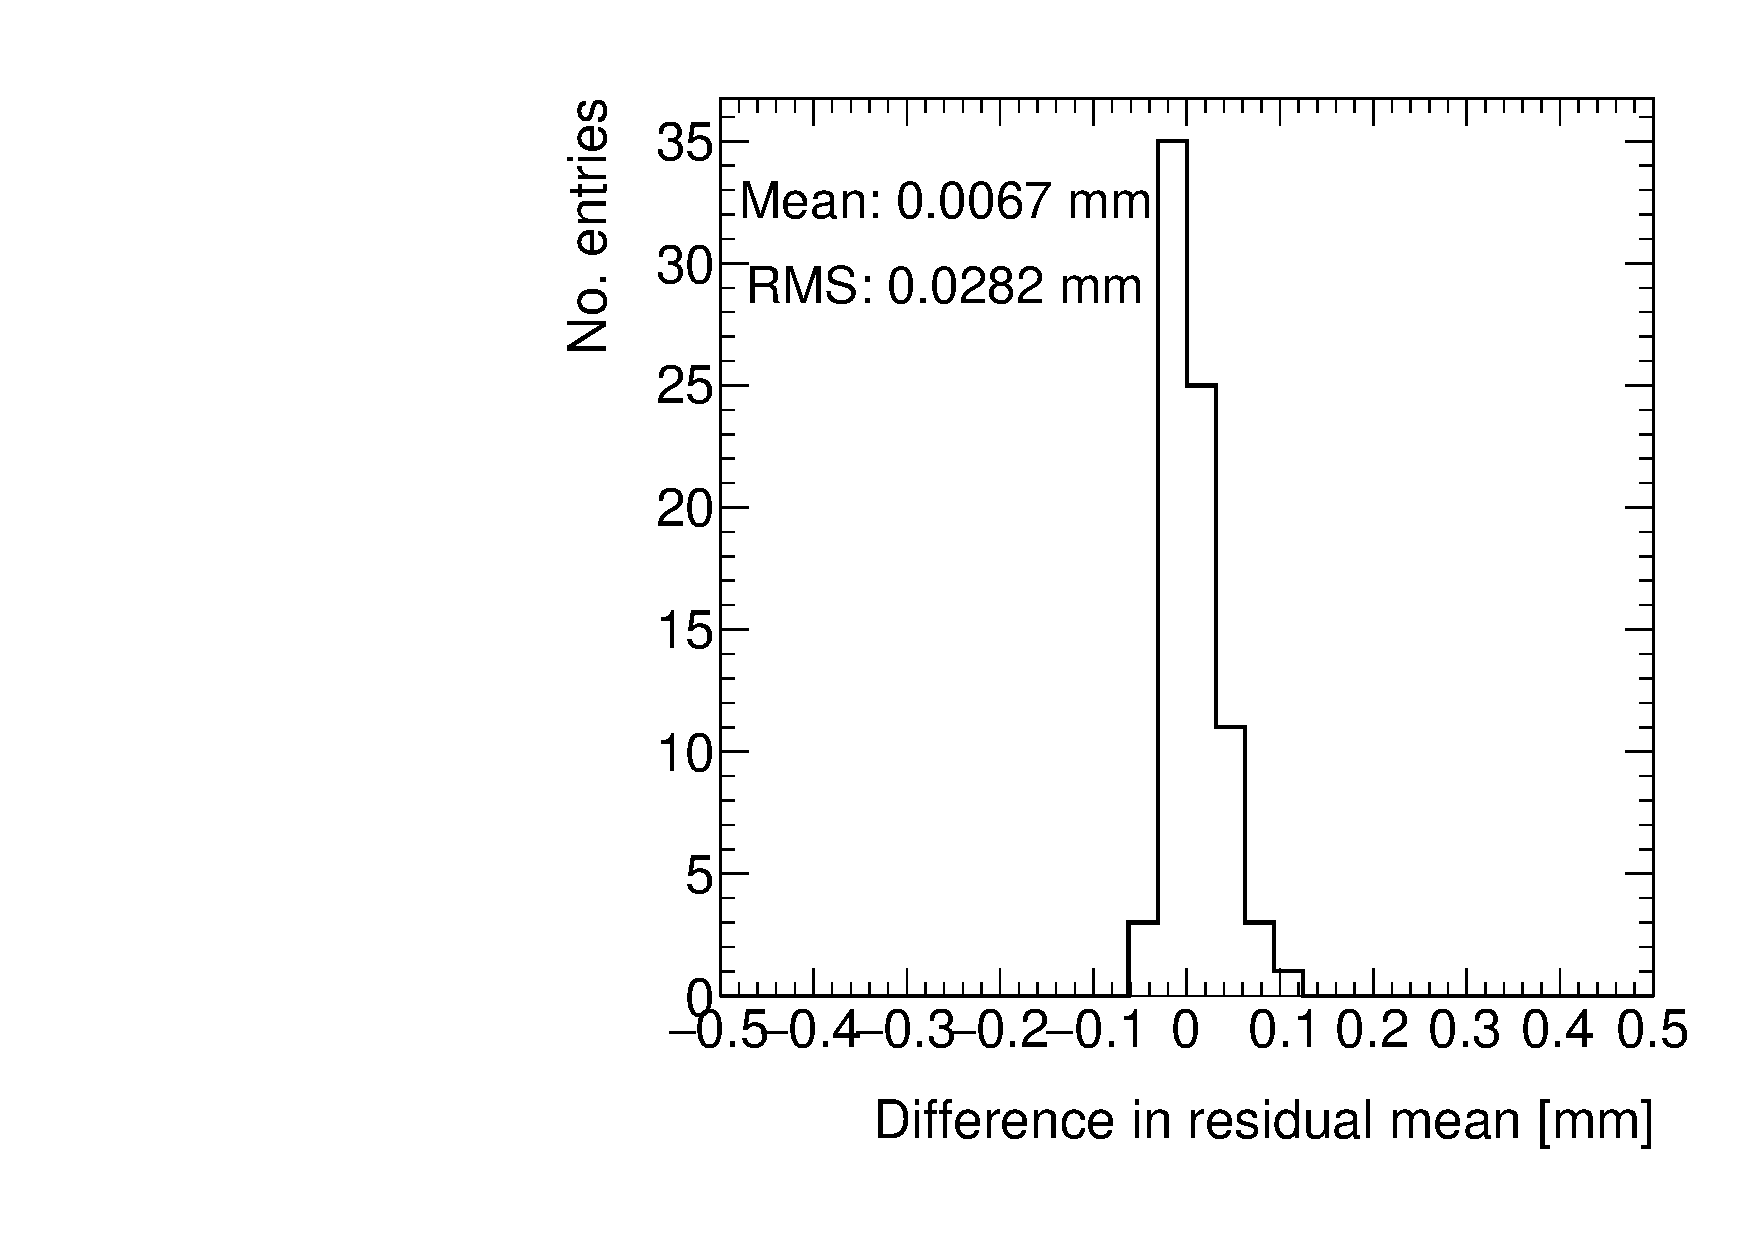
\includegraphics[width = 0.5\textwidth]{figures/compare_residual_fits_around_xrays_QL2C04_3100V_2021-05-20_100mm_bins_minus_QL2C04_3100V_2021-06-02_200mm_bins_means_difference.pdf}
    \caption{Difference in cosmic residual means around x-ray residuals for square bins of 100 mm width and 200 mm width for QL2.C.4.}
    \label{fig:area_bin_size_mean_diff}
\end{figure}

For this analysis, \SI{100}{\milli\meter} by \SI{100}{\milli\meter} bins were used.


